\documentclass[12pt]{article}

\usepackage{fullpage}
\usepackage{multicol,multirow}
\usepackage{tabularx}
\usepackage{ulem}
\usepackage[utf8]{inputenc}
\usepackage[russian]{babel}
\usepackage{color} %% это для отображения цвета в коде
\usepackage{listings} %% собственно, это и есть пакет listings
\usepackage{graphicx}%Вставка картинок правильная
\usepackage{float}%"Плавающие" картинки
\usepackage{wrapfig}%Обтекание фигур (таблиц, картинок и прочего)
\usepackage{caption}
\parindent=1cm
\DeclareCaptionFont{white}{\color{white}} %% это сделает текст заголовка белым
%% код ниже нарисует серую рамочку вокруг заголовка кода.
\DeclareCaptionFormat{listing}{\colorbox{gray}{\parbox{\textwidth}{#1#2#3}}}
\captionsetup[lstlisting]{format=listing,labelfont=white,textfont=white}

\begin{document}

\section*{Лабораторная работа №\,2 по курсу Криптография}

Выполнила студентка группы 08-307 МАИ \textit{Усачева Елизавета}.

\subsection*{Задание}

\begin{itemize}
    \item Создать пару OpenPGP-ключей, указав в сертификате свою почту.
    \item Установить связь с преподавателем, используя созданный ключ.
    \item Собрать подписи под своим сертификатом открытого ключа.
\end{itemize}

\subsection*{Введение}

OpenPGP – это открытый протокол шифрования электронной почты с использованием криптографии с открытым ключом. Он основан на оригинальном программном обеспечении PGP (Pretty Good Privacy). Протокол OpenPGP определяет стандартные форматы для зашифрованных сообщений, подписей и сертификатов для обмена открытыми ключами.

Шифрование OpenPGP может обеспечить безопасную доставку файлов и сообщений, а также обеспечить подтверждение того, кто создал или отправил сообщение, используя процесс, называемый цифровой подписью. Использование OpenPGP для связи требует участия как отправителя, так и получателя. OpenPGP также может использоваться для защиты конфиденциальных файлов, когда они хранятся в уязвимых местах, таких как мобильные устройства или в облаке.

\subsection*{Метод решения}

Для генерации публичного и приватного ключей и для подписания публичных ключей собеседников я использовала дополнение Enigmail для почтового клиента Thunderbird. Дополнение поддерживает шифрование, расшифровку и подпись электронных писем с использованием криптосистемы с открытым ключом PGP.

\begin{itemize}
    \item Установила связь с преподавателем и получила зашифрованное сообщение.
    \begin{figure}[h]
        \centering
        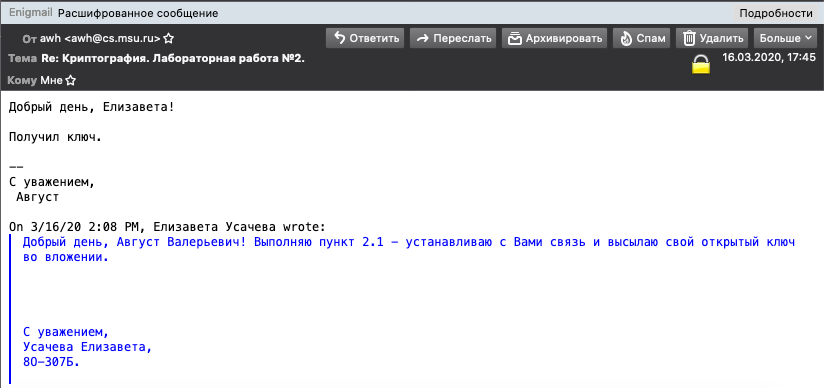
\includegraphics[width=0.8\linewidth]{1.png}
        %\caption{Диаграмма моментов на участке выбора момента прокатки}
        %\label{fig:mpr}
    \end{figure}
    \item Обменялась открытыми ключами с одногруппниками и собрала подпись.  \begin{figure}[h]
        \centering
        
\includegraphics[width=0.8\linewidth]{2.png}
        %\caption{Диаграмма моментов на участке выбора момента прокатки}
        %\label{fig:mpr}
    \end{figure}
\end{itemize}
    
\subsection*{Выводы}

В данной лабораторной работе я познакомилась с практическим шифрованием данных, предназначенным для безопасного обмена информацией и в качестве цифровой подписи. Однако, OpenPGP требует для связи участие обоих собеседников и личный контроль подлинности ключа шифрования собеседника, что является уязвимостью. 

\end{document}